\documentclass{tufte-handout}

%\date{28 March 2010} % without \date command, current date is supplied

%\geometry{showframe} % display margins for debugging page layout

\usepackage{graphicx} % allow embedded images
  \setkeys{Gin}{width=\linewidth,totalheight=\textheight,keepaspectratio}
  \graphicspath{{graphics/}} % set of paths to search for images
\usepackage{amsmath}  % extended mathematics
\usepackage{booktabs} % book-quality tables
\usepackage{units}    % non-stacked fractions and better unit spacing
\usepackage{multicol} % multiple column layout facilities
\usepackage{lipsum}   % filler text
\usepackage{fancyvrb} % extended verbatim environments
  \fvset{fontsize=\normalsize}% default font size for fancy-verbatim environments

% Standardize command font styles and environments
\newcommand{\doccmd}[1]{\texttt{\textbackslash#1}}% command name -- adds backslash automatically
\newcommand{\docopt}[1]{\ensuremath{\langle}\textrm{\textit{#1}}\ensuremath{\rangle}}% optional command argument
\newcommand{\docarg}[1]{\textrm{\textit{#1}}}% (required) command argument
\newcommand{\docenv}[1]{\textsf{#1}}% environment name
\newcommand{\docpkg}[1]{\texttt{#1}}% package name
\newcommand{\doccls}[1]{\texttt{#1}}% document class name
\newcommand{\docclsopt}[1]{\texttt{#1}}% document class option name
\newenvironment{docspec}{\begin{quote}\noindent}{\end{quote}}% command specification environment

\geometry{textwidth=.6\paperwidth}
\geometry{bottom=1.5cm}
\geometry{top=1.5cm}

\usepackage[utf8]{inputenc}
\usepackage{amssymb}

\newcommand{\Hau}{\text{Hau}}
\newcommand{\End}{\text{End}}
\newcommand{\inlinedef}[1]{\textcolor{purple}{#1}}
\newcommand{\id}{\text{id}}
\newcommand{\cf}{$\rightarrow$~}
\newcommand{\mat}[1]{\mathbf{#1}}


\usepackage{xcolor}

% \newenvironment{definition}[1]{
%  \colorbox{blue!30}{blue} \paragraph{#1}
% }{
%   .
% }


\newenvironment{definition}[2]{%
\par
\noindent
\paragraph{\colorbox{purple!30}{Def. #1}} (\textit{#2}) \\
\vspace{0.5em}
\noindent
}
{}


\newenvironment{exercise}[2]{%
  \par
  \noindent
  \paragraph{\colorbox{orange!30}{Ex. #1} ~ \textcolor{gray}{#2}} 
  \vspace{0.5em}
  \noindent
}{}

\newenvironment{theorem}[2]{%
  \par
  \noindent
  \paragraph{\colorbox{orange!30}{Th. #1}} (\textit{#2})\\
  \vspace{0.5em}
  \noindent
}{}

\newenvironment{algorithm}[2]{%
  \par
  \noindent
  \paragraph{\colorbox{blue!30}{Alg. #1}} (\textit{#2}) \\
  \vspace{0.5em}
  \noindent
}{}

\newenvironment{proof}{%
  \par
  \noindent
  \hfill\begin{minipage}{\dimexpr\textwidth-1em}
  \vspace{1em}
  \paragraph{Proof: }
  \noindent
}{
  \xdef\tpd{\the\prevdepth}
  \vspace{1em}
  \end{minipage}
}

\usepackage{enumitem}

\newcommand{\nn}{\ensuremath{\mathbb{N}}}

\newcommand{\len}{\ensuremath{\text{len}}}
\newcommand{\enc}{\ensuremath{\text{enc}}}
\newcommand{\leqae}{\ensuremath{\leq_{ae}}}

\newcommand{\twotdspace}{\textsc{2-t-dspace}}
\newcommand{\onetdspace}{\textsc{1-t-dspace}}

\newcommand{\bigO}{\ensuremath{\mathcal{O}}}


\makeatletter
\renewcommand{\paragraph}{%
  \@startsection{paragraph}{4}%
  {\z@}{0.00ex \@plus 1ex \@minus .2ex}{-1em}%
  {\normalfont\normalsize\bfseries}%
}
\makeatother

\begin{document}

\textsc{Multilevel Framework} --- User Manual

  \setlength{\parindent}{0em}
  \setlength{\parskip}{0.75em}

  \section{Introduction}
  \subsection{Overview}
  This Add-On provides a layout algorithm to \textsc{Vanted} that implements the
  multilevel graph layout framework. The user can select a \textit{merger}, a
  \textit{placer} and a \textit{layouter}, which will be applied as follows:
  \begin{enumerate}
  \item The \textit{merger} iteratively coarsens the graph, producing a number
    of levels of decreasing resolution.
  \item Starting from the most coarse level, each level is laid out using the
    given \textit{layout} algorithm.
  \item The resulting layout is then transferred to the level below using the
    \textit{placer}.
  \end{enumerate}

  \begin{figure}
    \centering
    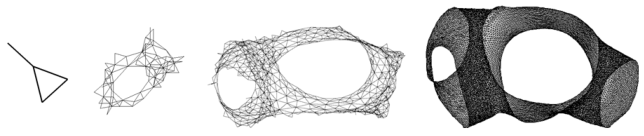
\includegraphics{coarsening}
    \caption{Increasingly coarse ``levels'' are constructed from the original
      graph from left to right. Then, from right to left, the graph is laid out,
    using the layout from the above level as a starting point.}
  \end{figure}

  \subsection{Dependencies}
  The plugin requires \textsc{Vanted} 2.6.5, including the libraries it is based upon.

  \subsection{License}
  Like \textsc{Vanted}
  \sidenote{\url{https://github.com/LSI-UniKonstanz/vanted/blob/master/src/main/resources/license.txt}}
  , this software is licensed under \textit{GNU General
    Public License, version 2}
  \sidenote[][1em]{\url{https://www.gnu.org/licenses/old-licenses/gpl-2.0.html}}.


  \section{Working with the Multilevel Framework}

  \subsection{Background}

  The merger builds multiple graphs (\textit{levels}) starting from the input
  graph. This process of creating representative graphs of decreasing size is
  known as \textit{coarsening} or \textit{merging}. During the merging process,
  several \textit{inner nodes} are merged into one \textit{merged node}. The
  merged node will be assigned coordinates to that it is centered between its
  inner nodes. The inner nodes can of course be merged nodes of lower coarsening
  levels.

  Starting with the smallest graph (the most coarse level), the chosen layout
  algorithm is applied. Then, the placer uses the layout of the next (less
  coarse) level to provide an initial layout for the current layouting step.
  Traversing downwards through all the levels from the coarsest to the finest
  level, which is the original graph, results in adjusted initial layouts for
  all layouting steps.

  \subsection{Limitations}
  \begin{itemize}
  \item The multilevel framework is meant to be used on undirected graphs.
    Directed graphs will be treated as if they are undirected.
  \item Only explicitly whitelisted layouting algorithms can be used.
  \end{itemize}

  \subsection{Options}

  \paragraph{Random layout for topmost layer} If checked, the topmost (most
  coarse) layer will be laid out randomly. If unchecked, the layout the layout
  of the topmost level is left unchanged. During construction of a level, merged
  nodes are placed centered relative to their inner nodes.

  \paragraph{Selection of layouter, merger and placer} Selecting a procedure the
  dropdown will display its parameter configuration below.

  \section{Mergers}

  \subsection{Random Merger}

  The random merger selects edges at random and merges the nodes that they connect (the
  edges are “collapsed”). 
 
  By default, it is not completely random, but prefers merging nodes
  with low weight (low number of nodes that they contain). It does this until a stop criterion
  (specified by the parameters described below) becomes true or no edges are left. The
  random merger stops at the first stop criterion that is hit.

  \paragraph{Coarsening Factor} Used to limit the number of edges that are
  actually merged. Other edges and their incident nodes are not touched and
  transferred without changes to the next level. For a graph with $n$ nodes and
  $m$ edges, the number of edges that will be coarsened is $c \cdot \min\{m,n\}$
  where $c$ is the selected coarsening factor. See below to see how edges are
  selected.

  \paragraph{Minimum number of nodes per level} The minimum number of nodes per
  level is a stop criterion for the random merger. If it finds that the number
  of nodes of the coarsening level that is currently being generated is less
  than or equal to this number, it will stop the coarsening process. 

  \paragraph{Maximum number of iterations} The absolute-valued counterpart to
  the coarsening factor. It describes a maximum number of merge operations that
  will be done for one level.

  \paragraph{Use merged-node weights} If selected and the coarsening factor is
  less than $1$, edges connecting merged nodes of low weight (i.e. containing
  few inner nodes) will be selected first for merging.

  \paragraph{Consider edge weights} If selected, edge weights of the given,
  bottom-most graph will be considered in the first coarsening step when
  selecting which edges to merge.

  \paragraph{Weight attribute path} This option determines the name of the edge
  weight attribute path that will be used if ``consider edge weights'' is
  enabled.

  \subsection{Solar Merger}
  The solar merger treats the graph and all the resulting smaller graphs as galaxies. The
  latter are a set of solar systems. Every node of the graph takes the role of a stellar body.
  There are three different types of bodies. Suns being the centers of their respective solar
  systems, planets which are nodes adjacent to their suns and moons which are neighbors of
  a planet but do not share edges to any sun.

  In each coarsening step, every solar system is “collapsed” into its sun. In this step, all
  edges between nodes of the collapsed systems are kept as edges between the resulting
  nodes. To fully take advantage of the Solar Merger, you should choose a placer which uses
  the solar system structure to place the nodes (the “Solar Placer”).

  In order to find solar systems for a graph (level), first the graph has to be
  partitioned. This is done by determining a set of suns. Using a candidate set
  containing all nodes, a random node is marked as a sun. The sun and the nodes
  which are one and two edge-hops away are removed from the candidate set. This is
  done until there are no candidates left.

  The set of suns is then used to set up solar systems. For each of the suns,
  its direct neighbors are marked as planets belonging to their sun. The remaining
  nodes, which are neither sun nor planet, are marked as moons with a single
  planet next to them as their planet. As a result all nodes of the Graph have a
  role (sun, planet or moon) and a corresponding solar system.

  Finally, nodes and edges for the next level have to be created. For every
  solar system of the galaxy, the sun, all planets and moons are added as inner
  nodes to a merged node in the new graph. If one of the inner nodes had an edge
  to an inner node of another solar system an edge is created between the two
  new nodes.

  This is done until one of the termination criteria is fulfilled.

  \paragraph{Minimum number of nodes} When the number of nodes of the
  graph/subgraph is lower than the given value, the Solar Merger stops.

  \paragraph{Maximum level factor} Limits how many times a new galaxy is
  created or, in other words, how many levels are generated. The size of the
  original graph divided by the maximum level factor is used as the maximum
  amount of levels.

  \section{Placers}

  \subsection{Random Placer}

  The random placer places noes randomly within a given radius around the merged node.

  \paragraph{Maximum place distance} The radius within which the Random Placer
  places the nodes can be configured. If the layout algorithm you chose has a
  target edge length or a minimum edge length, a reasonable value for the radius
  option would be half of this length.

  \subsection{Solar Placer}

  The Solar Placer is the correspondent placer to the Solar Merger. It uses to
  the structure of solar systems to create promising initial layouts for the
  layouters. The placement is done by placing the sun for every solar system at
  position of the node representing the solar system in the smaller graph.

  Planets which do not have neighbors in other solar systems and no moons with
  neighbors in other solar systems are placed randomly around the sun. Moons
  which do not have neighbors in other solar systems are placed randomly around
  their planets. Planets and moons which have neighbors in other solar systems
  are placed on a path between these solar systems’ suns. The planets and moons
  on such a path are placed equidistantly on a line between these suns.

  There are no options available.
  

\end{document}
